% Created by tikzDevice version 0.7.0 on 2015-05-17 06:40:04
% !TEX encoding = UTF-8 Unicode
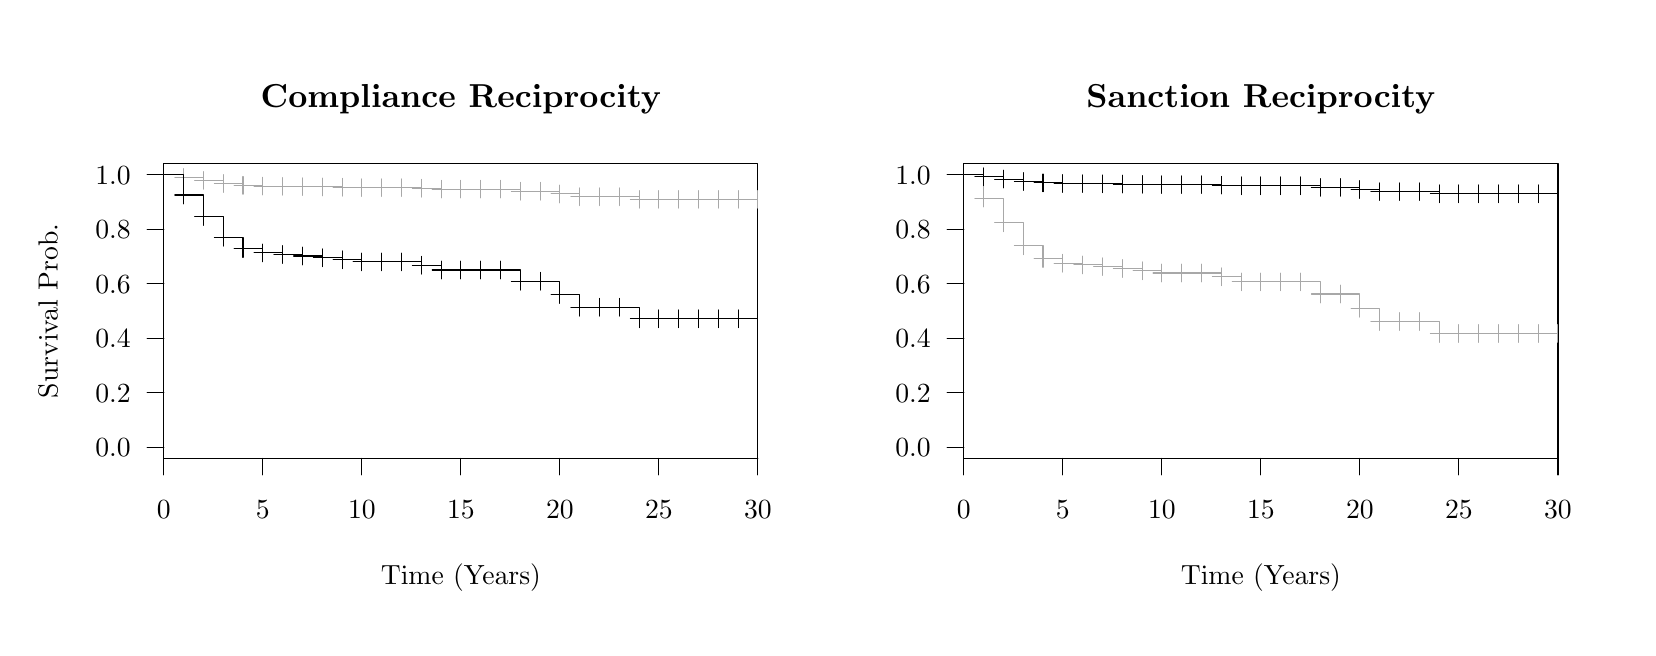
\begin{tikzpicture}[x=1pt,y=1pt]
\definecolor[named]{fillColor}{rgb}{1.00,1.00,1.00}
\path[use as bounding box,fill=fillColor,fill opacity=0.00] (0,0) rectangle (578.16,216.81);
\begin{scope}
\path[clip] (  0.00,  0.00) rectangle (578.16,216.81);
\definecolor[named]{drawColor}{rgb}{0.00,0.00,0.00}

\path[draw=drawColor,line width= 0.4pt,line join=round,line cap=round] ( 49.20, 61.20) -- (263.88, 61.20);

\path[draw=drawColor,line width= 0.4pt,line join=round,line cap=round] ( 49.20, 61.20) -- ( 49.20, 55.20);

\path[draw=drawColor,line width= 0.4pt,line join=round,line cap=round] ( 84.98, 61.20) -- ( 84.98, 55.20);

\path[draw=drawColor,line width= 0.4pt,line join=round,line cap=round] (120.76, 61.20) -- (120.76, 55.20);

\path[draw=drawColor,line width= 0.4pt,line join=round,line cap=round] (156.54, 61.20) -- (156.54, 55.20);

\path[draw=drawColor,line width= 0.4pt,line join=round,line cap=round] (192.32, 61.20) -- (192.32, 55.20);

\path[draw=drawColor,line width= 0.4pt,line join=round,line cap=round] (228.10, 61.20) -- (228.10, 55.20);

\path[draw=drawColor,line width= 0.4pt,line join=round,line cap=round] (263.88, 61.20) -- (263.88, 55.20);

\node[text=drawColor,anchor=base,inner sep=0pt, outer sep=0pt, scale=  1.00] at ( 49.20, 39.60) {0};

\node[text=drawColor,anchor=base,inner sep=0pt, outer sep=0pt, scale=  1.00] at ( 84.98, 39.60) {5};

\node[text=drawColor,anchor=base,inner sep=0pt, outer sep=0pt, scale=  1.00] at (120.76, 39.60) {10};

\node[text=drawColor,anchor=base,inner sep=0pt, outer sep=0pt, scale=  1.00] at (156.54, 39.60) {15};

\node[text=drawColor,anchor=base,inner sep=0pt, outer sep=0pt, scale=  1.00] at (192.32, 39.60) {20};

\node[text=drawColor,anchor=base,inner sep=0pt, outer sep=0pt, scale=  1.00] at (228.10, 39.60) {25};

\node[text=drawColor,anchor=base,inner sep=0pt, outer sep=0pt, scale=  1.00] at (263.88, 39.60) {30};

\path[draw=drawColor,line width= 0.4pt,line join=round,line cap=round] ( 49.20, 65.14) -- ( 49.20,163.67);

\path[draw=drawColor,line width= 0.4pt,line join=round,line cap=round] ( 49.20, 65.14) -- ( 43.20, 65.14);

\path[draw=drawColor,line width= 0.4pt,line join=round,line cap=round] ( 49.20, 84.85) -- ( 43.20, 84.85);

\path[draw=drawColor,line width= 0.4pt,line join=round,line cap=round] ( 49.20,104.55) -- ( 43.20,104.55);

\path[draw=drawColor,line width= 0.4pt,line join=round,line cap=round] ( 49.20,124.26) -- ( 43.20,124.26);

\path[draw=drawColor,line width= 0.4pt,line join=round,line cap=round] ( 49.20,143.96) -- ( 43.20,143.96);

\path[draw=drawColor,line width= 0.4pt,line join=round,line cap=round] ( 49.20,163.67) -- ( 43.20,163.67);

\node[text=drawColor,anchor=base east,inner sep=0pt, outer sep=0pt, scale=  1.00] at ( 37.20, 61.70) {0.0};

\node[text=drawColor,anchor=base east,inner sep=0pt, outer sep=0pt, scale=  1.00] at ( 37.20, 81.40) {0.2};

\node[text=drawColor,anchor=base east,inner sep=0pt, outer sep=0pt, scale=  1.00] at ( 37.20,101.11) {0.4};

\node[text=drawColor,anchor=base east,inner sep=0pt, outer sep=0pt, scale=  1.00] at ( 37.20,120.81) {0.6};

\node[text=drawColor,anchor=base east,inner sep=0pt, outer sep=0pt, scale=  1.00] at ( 37.20,140.52) {0.8};

\node[text=drawColor,anchor=base east,inner sep=0pt, outer sep=0pt, scale=  1.00] at ( 37.20,160.23) {1.0};

\path[draw=drawColor,line width= 0.4pt,line join=round,line cap=round] ( 49.20, 61.20) --
	(263.88, 61.20) --
	(263.88,167.61) --
	( 49.20,167.61) --
	( 49.20, 61.20);
\end{scope}
\begin{scope}
\path[clip] (  0.00,  0.00) rectangle (289.08,216.81);
\definecolor[named]{drawColor}{rgb}{0.00,0.00,0.00}

\node[text=drawColor,anchor=base,inner sep=0pt, outer sep=0pt, scale=  1.20] at (156.54,188.07) {\bfseries Compliance Reciprocity};
\end{scope}
\begin{scope}
\path[clip] ( 49.20, 61.20) rectangle (263.88,167.61);
\definecolor[named]{drawColor}{rgb}{0.66,0.66,0.66}

\path[draw=drawColor,line width= 0.4pt,line join=round,line cap=round] ( 49.20,163.67) --
	( 56.36,163.67) --
	( 56.36,162.71) --
	( 63.51,162.71) --
	( 63.51,161.62) --
	( 70.67,161.62) --
	( 70.67,160.49) --
	( 77.82,160.49) --
	( 77.82,159.82) --
	( 84.98,159.82) --
	( 84.98,159.56) --
	( 92.14,159.56) --
	( 92.14,159.47) --
	( 99.29,159.47) --
	( 99.29,159.37) --
	(106.45,159.37) --
	(106.45,159.26) --
	(113.60,159.26) --
	(113.60,159.13) --
	(120.76,159.13) --
	(120.76,159.00) --
	(142.23,159.00) --
	(142.23,158.78) --
	(149.38,158.78) --
	(149.38,158.47) --
	(178.01,158.47) --
	(178.01,157.71) --
	(192.32,157.71) --
	(192.32,156.73) --
	(199.48,156.73) --
	(199.48,155.74) --
	(220.94,155.74) --
	(220.94,154.76) --
	(464.25,154.76) --
	(464.25,154.76);

\path[draw=drawColor,line width= 0.4pt,line join=round,line cap=round] ( 53.17,162.71) -- ( 59.54,162.71);

\path[draw=drawColor,line width= 0.4pt,line join=round,line cap=round] ( 56.36,159.53) -- ( 56.36,165.90);

\path[draw=drawColor,line width= 0.4pt,line join=round,line cap=round] ( 60.33,161.62) -- ( 66.69,161.62);

\path[draw=drawColor,line width= 0.4pt,line join=round,line cap=round] ( 63.51,158.44) -- ( 63.51,164.80);

\path[draw=drawColor,line width= 0.4pt,line join=round,line cap=round] ( 67.49,160.49) -- ( 73.85,160.49);

\path[draw=drawColor,line width= 0.4pt,line join=round,line cap=round] ( 70.67,157.30) -- ( 70.67,163.67);

\path[draw=drawColor,line width= 0.4pt,line join=round,line cap=round] ( 74.64,159.82) -- ( 81.01,159.82);

\path[draw=drawColor,line width= 0.4pt,line join=round,line cap=round] ( 77.82,156.64) -- ( 77.82,163.01);

\path[draw=drawColor,line width= 0.4pt,line join=round,line cap=round] ( 81.80,159.56) -- ( 88.16,159.56);

\path[draw=drawColor,line width= 0.4pt,line join=round,line cap=round] ( 84.98,156.38) -- ( 84.98,162.74);

\path[draw=drawColor,line width= 0.4pt,line join=round,line cap=round] ( 88.95,159.47) -- ( 95.32,159.47);

\path[draw=drawColor,line width= 0.4pt,line join=round,line cap=round] ( 92.14,156.28) -- ( 92.14,162.65);

\path[draw=drawColor,line width= 0.4pt,line join=round,line cap=round] ( 96.11,159.37) -- (102.47,159.37);

\path[draw=drawColor,line width= 0.4pt,line join=round,line cap=round] ( 99.29,156.19) -- ( 99.29,162.55);

\path[draw=drawColor,line width= 0.4pt,line join=round,line cap=round] (103.27,159.26) -- (109.63,159.26);

\path[draw=drawColor,line width= 0.4pt,line join=round,line cap=round] (106.45,156.08) -- (106.45,162.44);

\path[draw=drawColor,line width= 0.4pt,line join=round,line cap=round] (110.42,159.13) -- (116.79,159.13);

\path[draw=drawColor,line width= 0.4pt,line join=round,line cap=round] (113.60,155.95) -- (113.60,162.31);

\path[draw=drawColor,line width= 0.4pt,line join=round,line cap=round] (117.58,159.00) -- (123.94,159.00);

\path[draw=drawColor,line width= 0.4pt,line join=round,line cap=round] (120.76,155.82) -- (120.76,162.18);

\path[draw=drawColor,line width= 0.4pt,line join=round,line cap=round] (124.73,159.00) -- (131.10,159.00);

\path[draw=drawColor,line width= 0.4pt,line join=round,line cap=round] (127.92,155.82) -- (127.92,162.18);

\path[draw=drawColor,line width= 0.4pt,line join=round,line cap=round] (131.89,159.00) -- (138.25,159.00);

\path[draw=drawColor,line width= 0.4pt,line join=round,line cap=round] (135.07,155.82) -- (135.07,162.18);

\path[draw=drawColor,line width= 0.4pt,line join=round,line cap=round] (139.05,158.78) -- (145.41,158.78);

\path[draw=drawColor,line width= 0.4pt,line join=round,line cap=round] (142.23,155.60) -- (142.23,161.97);

\path[draw=drawColor,line width= 0.4pt,line join=round,line cap=round] (146.20,158.47) -- (152.57,158.47);

\path[draw=drawColor,line width= 0.4pt,line join=round,line cap=round] (149.38,155.29) -- (149.38,161.65);

\path[draw=drawColor,line width= 0.4pt,line join=round,line cap=round] (153.36,158.47) -- (159.72,158.47);

\path[draw=drawColor,line width= 0.4pt,line join=round,line cap=round] (156.54,155.29) -- (156.54,161.65);

\path[draw=drawColor,line width= 0.4pt,line join=round,line cap=round] (160.51,158.47) -- (166.88,158.47);

\path[draw=drawColor,line width= 0.4pt,line join=round,line cap=round] (163.70,155.29) -- (163.70,161.65);

\path[draw=drawColor,line width= 0.4pt,line join=round,line cap=round] (167.67,158.47) -- (174.03,158.47);

\path[draw=drawColor,line width= 0.4pt,line join=round,line cap=round] (170.85,155.29) -- (170.85,161.65);

\path[draw=drawColor,line width= 0.4pt,line join=round,line cap=round] (174.83,157.71) -- (181.19,157.71);

\path[draw=drawColor,line width= 0.4pt,line join=round,line cap=round] (178.01,154.52) -- (178.01,160.89);

\path[draw=drawColor,line width= 0.4pt,line join=round,line cap=round] (181.98,157.71) -- (188.35,157.71);

\path[draw=drawColor,line width= 0.4pt,line join=round,line cap=round] (185.16,154.52) -- (185.16,160.89);

\path[draw=drawColor,line width= 0.4pt,line join=round,line cap=round] (189.14,156.73) -- (195.50,156.73);

\path[draw=drawColor,line width= 0.4pt,line join=round,line cap=round] (192.32,153.55) -- (192.32,159.91);

\path[draw=drawColor,line width= 0.4pt,line join=round,line cap=round] (196.29,155.74) -- (202.66,155.74);

\path[draw=drawColor,line width= 0.4pt,line join=round,line cap=round] (199.48,152.56) -- (199.48,158.92);

\path[draw=drawColor,line width= 0.4pt,line join=round,line cap=round] (203.45,155.74) -- (209.81,155.74);

\path[draw=drawColor,line width= 0.4pt,line join=round,line cap=round] (206.63,152.56) -- (206.63,158.92);

\path[draw=drawColor,line width= 0.4pt,line join=round,line cap=round] (210.61,155.74) -- (216.97,155.74);

\path[draw=drawColor,line width= 0.4pt,line join=round,line cap=round] (213.79,152.56) -- (213.79,158.92);

\path[draw=drawColor,line width= 0.4pt,line join=round,line cap=round] (217.76,154.76) -- (224.13,154.76);

\path[draw=drawColor,line width= 0.4pt,line join=round,line cap=round] (220.94,151.58) -- (220.94,157.95);

\path[draw=drawColor,line width= 0.4pt,line join=round,line cap=round] (224.92,154.76) -- (231.28,154.76);

\path[draw=drawColor,line width= 0.4pt,line join=round,line cap=round] (228.10,151.58) -- (228.10,157.95);

\path[draw=drawColor,line width= 0.4pt,line join=round,line cap=round] (232.07,154.76) -- (238.44,154.76);

\path[draw=drawColor,line width= 0.4pt,line join=round,line cap=round] (235.26,151.58) -- (235.26,157.95);

\path[draw=drawColor,line width= 0.4pt,line join=round,line cap=round] (239.23,154.76) -- (245.59,154.76);

\path[draw=drawColor,line width= 0.4pt,line join=round,line cap=round] (242.41,151.58) -- (242.41,157.95);

\path[draw=drawColor,line width= 0.4pt,line join=round,line cap=round] (246.39,154.76) -- (252.75,154.76);

\path[draw=drawColor,line width= 0.4pt,line join=round,line cap=round] (249.57,151.58) -- (249.57,157.95);

\path[draw=drawColor,line width= 0.4pt,line join=round,line cap=round] (253.54,154.76) -- (259.91,154.76);

\path[draw=drawColor,line width= 0.4pt,line join=round,line cap=round] (256.72,151.58) -- (256.72,157.95);

\path[draw=drawColor,line width= 0.4pt,line join=round,line cap=round] (260.70,154.76) -- (267.06,154.76);

\path[draw=drawColor,line width= 0.4pt,line join=round,line cap=round] (263.88,151.58) -- (263.88,157.95);

\path[draw=drawColor,line width= 0.4pt,line join=round,line cap=round] (267.85,154.76) -- (274.22,154.76);

\path[draw=drawColor,line width= 0.4pt,line join=round,line cap=round] (271.04,151.58) -- (271.04,157.95);

\path[draw=drawColor,line width= 0.4pt,line join=round,line cap=round] (275.01,154.76) -- (281.37,154.76);

\path[draw=drawColor,line width= 0.4pt,line join=round,line cap=round] (278.19,151.58) -- (278.19,157.95);

\path[draw=drawColor,line width= 0.4pt,line join=round,line cap=round] (282.17,154.76) -- (288.53,154.76);

\path[draw=drawColor,line width= 0.4pt,line join=round,line cap=round] (285.35,151.58) -- (285.35,157.95);

\path[draw=drawColor,line width= 0.4pt,line join=round,line cap=round] (289.32,154.76) -- (295.69,154.76);

\path[draw=drawColor,line width= 0.4pt,line join=round,line cap=round] (292.50,151.58) -- (292.50,157.95);

\path[draw=drawColor,line width= 0.4pt,line join=round,line cap=round] (296.48,154.76) -- (302.84,154.76);

\path[draw=drawColor,line width= 0.4pt,line join=round,line cap=round] (299.66,151.58) -- (299.66,157.95);

\path[draw=drawColor,line width= 0.4pt,line join=round,line cap=round] (303.63,154.76) -- (310.00,154.76);

\path[draw=drawColor,line width= 0.4pt,line join=round,line cap=round] (306.82,151.58) -- (306.82,157.95);

\path[draw=drawColor,line width= 0.4pt,line join=round,line cap=round] (310.79,154.76) -- (317.15,154.76);

\path[draw=drawColor,line width= 0.4pt,line join=round,line cap=round] (313.97,151.58) -- (313.97,157.95);

\path[draw=drawColor,line width= 0.4pt,line join=round,line cap=round] (317.95,154.76) -- (324.31,154.76);

\path[draw=drawColor,line width= 0.4pt,line join=round,line cap=round] (321.13,151.58) -- (321.13,157.95);

\path[draw=drawColor,line width= 0.4pt,line join=round,line cap=round] (325.10,154.76) -- (331.47,154.76);

\path[draw=drawColor,line width= 0.4pt,line join=round,line cap=round] (328.28,151.58) -- (328.28,157.95);

\path[draw=drawColor,line width= 0.4pt,line join=round,line cap=round] (332.26,154.76) -- (338.62,154.76);

\path[draw=drawColor,line width= 0.4pt,line join=round,line cap=round] (335.44,151.58) -- (335.44,157.95);

\path[draw=drawColor,line width= 0.4pt,line join=round,line cap=round] (339.41,154.76) -- (345.78,154.76);

\path[draw=drawColor,line width= 0.4pt,line join=round,line cap=round] (342.60,151.58) -- (342.60,157.95);

\path[draw=drawColor,line width= 0.4pt,line join=round,line cap=round] (346.57,154.76) -- (352.93,154.76);

\path[draw=drawColor,line width= 0.4pt,line join=round,line cap=round] (349.75,151.58) -- (349.75,157.95);

\path[draw=drawColor,line width= 0.4pt,line join=round,line cap=round] (353.73,154.76) -- (360.09,154.76);

\path[draw=drawColor,line width= 0.4pt,line join=round,line cap=round] (356.91,151.58) -- (356.91,157.95);

\path[draw=drawColor,line width= 0.4pt,line join=round,line cap=round] (360.88,154.76) -- (367.25,154.76);

\path[draw=drawColor,line width= 0.4pt,line join=round,line cap=round] (364.06,151.58) -- (364.06,157.95);

\path[draw=drawColor,line width= 0.4pt,line join=round,line cap=round] (368.04,154.76) -- (374.40,154.76);

\path[draw=drawColor,line width= 0.4pt,line join=round,line cap=round] (371.22,151.58) -- (371.22,157.95);

\path[draw=drawColor,line width= 0.4pt,line join=round,line cap=round] (375.19,154.76) -- (381.56,154.76);

\path[draw=drawColor,line width= 0.4pt,line join=round,line cap=round] (378.38,151.58) -- (378.38,157.95);

\path[draw=drawColor,line width= 0.4pt,line join=round,line cap=round] (382.35,154.76) -- (388.71,154.76);

\path[draw=drawColor,line width= 0.4pt,line join=round,line cap=round] (385.53,151.58) -- (385.53,157.95);

\path[draw=drawColor,line width= 0.4pt,line join=round,line cap=round] (389.51,154.76) -- (395.87,154.76);

\path[draw=drawColor,line width= 0.4pt,line join=round,line cap=round] (392.69,151.58) -- (392.69,157.95);

\path[draw=drawColor,line width= 0.4pt,line join=round,line cap=round] (396.66,154.76) -- (403.03,154.76);

\path[draw=drawColor,line width= 0.4pt,line join=round,line cap=round] (399.84,151.58) -- (399.84,157.95);

\path[draw=drawColor,line width= 0.4pt,line join=round,line cap=round] (403.82,154.76) -- (410.18,154.76);

\path[draw=drawColor,line width= 0.4pt,line join=round,line cap=round] (407.00,151.58) -- (407.00,157.95);

\path[draw=drawColor,line width= 0.4pt,line join=round,line cap=round] (410.97,154.76) -- (417.34,154.76);

\path[draw=drawColor,line width= 0.4pt,line join=round,line cap=round] (414.16,151.58) -- (414.16,157.95);

\path[draw=drawColor,line width= 0.4pt,line join=round,line cap=round] (418.13,154.76) -- (424.49,154.76);

\path[draw=drawColor,line width= 0.4pt,line join=round,line cap=round] (421.31,151.58) -- (421.31,157.95);

\path[draw=drawColor,line width= 0.4pt,line join=round,line cap=round] (425.29,154.76) -- (431.65,154.76);

\path[draw=drawColor,line width= 0.4pt,line join=round,line cap=round] (428.47,151.58) -- (428.47,157.95);

\path[draw=drawColor,line width= 0.4pt,line join=round,line cap=round] (432.44,154.76) -- (438.81,154.76);

\path[draw=drawColor,line width= 0.4pt,line join=round,line cap=round] (435.62,151.58) -- (435.62,157.95);

\path[draw=drawColor,line width= 0.4pt,line join=round,line cap=round] (439.60,154.76) -- (445.96,154.76);

\path[draw=drawColor,line width= 0.4pt,line join=round,line cap=round] (442.78,151.58) -- (442.78,157.95);

\path[draw=drawColor,line width= 0.4pt,line join=round,line cap=round] (446.75,154.76) -- (453.12,154.76);

\path[draw=drawColor,line width= 0.4pt,line join=round,line cap=round] (449.94,151.58) -- (449.94,157.95);

\path[draw=drawColor,line width= 0.4pt,line join=round,line cap=round] (453.91,154.76) -- (460.27,154.76);

\path[draw=drawColor,line width= 0.4pt,line join=round,line cap=round] (457.09,151.58) -- (457.09,157.95);

\path[draw=drawColor,line width= 0.4pt,line join=round,line cap=round] (461.07,154.76) -- (467.43,154.76);

\path[draw=drawColor,line width= 0.4pt,line join=round,line cap=round] (464.25,151.58) -- (464.25,157.95);
\definecolor[named]{drawColor}{rgb}{0.00,0.00,0.00}

\path[draw=drawColor,line width= 0.4pt,line join=round,line cap=round] ( 49.20,163.67) --
	( 56.36,163.67) --
	( 56.36,156.34) --
	( 63.51,156.34) --
	( 63.51,148.53) --
	( 70.67,148.53) --
	( 70.67,141.08) --
	( 77.82,141.08) --
	( 77.82,136.99) --
	( 84.98,136.99) --
	( 84.98,135.42) --
	( 92.14,135.42) --
	( 92.14,134.87) --
	( 99.29,134.87) --
	( 99.29,134.31) --
	(106.45,134.31) --
	(106.45,133.67) --
	(113.60,133.67) --
	(113.60,132.94) --
	(120.76,132.94) --
	(120.76,132.18) --
	(142.23,132.18) --
	(142.23,130.97) --
	(149.38,130.97) --
	(149.38,129.25) --
	(178.01,129.25) --
	(178.01,125.19) --
	(192.32,125.19) --
	(192.32,120.36) --
	(199.48,120.36) --
	(199.48,115.80) --
	(220.94,115.80) --
	(220.94,111.63) --
	(464.25,111.63) --
	(464.25,111.63);

\path[draw=drawColor,line width= 0.4pt,line join=round,line cap=round] ( 53.17,156.34) -- ( 59.54,156.34);

\path[draw=drawColor,line width= 0.4pt,line join=round,line cap=round] ( 56.36,153.16) -- ( 56.36,159.52);

\path[draw=drawColor,line width= 0.4pt,line join=round,line cap=round] ( 60.33,148.53) -- ( 66.69,148.53);

\path[draw=drawColor,line width= 0.4pt,line join=round,line cap=round] ( 63.51,145.35) -- ( 63.51,151.71);

\path[draw=drawColor,line width= 0.4pt,line join=round,line cap=round] ( 67.49,141.08) -- ( 73.85,141.08);

\path[draw=drawColor,line width= 0.4pt,line join=round,line cap=round] ( 70.67,137.90) -- ( 70.67,144.26);

\path[draw=drawColor,line width= 0.4pt,line join=round,line cap=round] ( 74.64,136.99) -- ( 81.01,136.99);

\path[draw=drawColor,line width= 0.4pt,line join=round,line cap=round] ( 77.82,133.81) -- ( 77.82,140.17);

\path[draw=drawColor,line width= 0.4pt,line join=round,line cap=round] ( 81.80,135.42) -- ( 88.16,135.42);

\path[draw=drawColor,line width= 0.4pt,line join=round,line cap=round] ( 84.98,132.24) -- ( 84.98,138.60);

\path[draw=drawColor,line width= 0.4pt,line join=round,line cap=round] ( 88.95,134.87) -- ( 95.32,134.87);

\path[draw=drawColor,line width= 0.4pt,line join=round,line cap=round] ( 92.14,131.68) -- ( 92.14,138.05);

\path[draw=drawColor,line width= 0.4pt,line join=round,line cap=round] ( 96.11,134.31) -- (102.47,134.31);

\path[draw=drawColor,line width= 0.4pt,line join=round,line cap=round] ( 99.29,131.13) -- ( 99.29,137.49);

\path[draw=drawColor,line width= 0.4pt,line join=round,line cap=round] (103.27,133.67) -- (109.63,133.67);

\path[draw=drawColor,line width= 0.4pt,line join=round,line cap=round] (106.45,130.49) -- (106.45,136.85);

\path[draw=drawColor,line width= 0.4pt,line join=round,line cap=round] (110.42,132.94) -- (116.79,132.94);

\path[draw=drawColor,line width= 0.4pt,line join=round,line cap=round] (113.60,129.75) -- (113.60,136.12);

\path[draw=drawColor,line width= 0.4pt,line join=round,line cap=round] (117.58,132.18) -- (123.94,132.18);

\path[draw=drawColor,line width= 0.4pt,line join=round,line cap=round] (120.76,128.99) -- (120.76,135.36);

\path[draw=drawColor,line width= 0.4pt,line join=round,line cap=round] (124.73,132.18) -- (131.10,132.18);

\path[draw=drawColor,line width= 0.4pt,line join=round,line cap=round] (127.92,128.99) -- (127.92,135.36);

\path[draw=drawColor,line width= 0.4pt,line join=round,line cap=round] (131.89,132.18) -- (138.25,132.18);

\path[draw=drawColor,line width= 0.4pt,line join=round,line cap=round] (135.07,128.99) -- (135.07,135.36);

\path[draw=drawColor,line width= 0.4pt,line join=round,line cap=round] (139.05,130.97) -- (145.41,130.97);

\path[draw=drawColor,line width= 0.4pt,line join=round,line cap=round] (142.23,127.79) -- (142.23,134.15);

\path[draw=drawColor,line width= 0.4pt,line join=round,line cap=round] (146.20,129.25) -- (152.57,129.25);

\path[draw=drawColor,line width= 0.4pt,line join=round,line cap=round] (149.38,126.06) -- (149.38,132.43);

\path[draw=drawColor,line width= 0.4pt,line join=round,line cap=round] (153.36,129.25) -- (159.72,129.25);

\path[draw=drawColor,line width= 0.4pt,line join=round,line cap=round] (156.54,126.06) -- (156.54,132.43);

\path[draw=drawColor,line width= 0.4pt,line join=round,line cap=round] (160.51,129.25) -- (166.88,129.25);

\path[draw=drawColor,line width= 0.4pt,line join=round,line cap=round] (163.70,126.06) -- (163.70,132.43);

\path[draw=drawColor,line width= 0.4pt,line join=round,line cap=round] (167.67,129.25) -- (174.03,129.25);

\path[draw=drawColor,line width= 0.4pt,line join=round,line cap=round] (170.85,126.06) -- (170.85,132.43);

\path[draw=drawColor,line width= 0.4pt,line join=round,line cap=round] (174.83,125.19) -- (181.19,125.19);

\path[draw=drawColor,line width= 0.4pt,line join=round,line cap=round] (178.01,122.01) -- (178.01,128.38);

\path[draw=drawColor,line width= 0.4pt,line join=round,line cap=round] (181.98,125.19) -- (188.35,125.19);

\path[draw=drawColor,line width= 0.4pt,line join=round,line cap=round] (185.16,122.01) -- (185.16,128.38);

\path[draw=drawColor,line width= 0.4pt,line join=round,line cap=round] (189.14,120.36) -- (195.50,120.36);

\path[draw=drawColor,line width= 0.4pt,line join=round,line cap=round] (192.32,117.18) -- (192.32,123.54);

\path[draw=drawColor,line width= 0.4pt,line join=round,line cap=round] (196.29,115.80) -- (202.66,115.80);

\path[draw=drawColor,line width= 0.4pt,line join=round,line cap=round] (199.48,112.62) -- (199.48,118.99);

\path[draw=drawColor,line width= 0.4pt,line join=round,line cap=round] (203.45,115.80) -- (209.81,115.80);

\path[draw=drawColor,line width= 0.4pt,line join=round,line cap=round] (206.63,112.62) -- (206.63,118.99);

\path[draw=drawColor,line width= 0.4pt,line join=round,line cap=round] (210.61,115.80) -- (216.97,115.80);

\path[draw=drawColor,line width= 0.4pt,line join=round,line cap=round] (213.79,112.62) -- (213.79,118.99);

\path[draw=drawColor,line width= 0.4pt,line join=round,line cap=round] (217.76,111.63) -- (224.13,111.63);

\path[draw=drawColor,line width= 0.4pt,line join=round,line cap=round] (220.94,108.44) -- (220.94,114.81);

\path[draw=drawColor,line width= 0.4pt,line join=round,line cap=round] (224.92,111.63) -- (231.28,111.63);

\path[draw=drawColor,line width= 0.4pt,line join=round,line cap=round] (228.10,108.44) -- (228.10,114.81);

\path[draw=drawColor,line width= 0.4pt,line join=round,line cap=round] (232.07,111.63) -- (238.44,111.63);

\path[draw=drawColor,line width= 0.4pt,line join=round,line cap=round] (235.26,108.44) -- (235.26,114.81);

\path[draw=drawColor,line width= 0.4pt,line join=round,line cap=round] (239.23,111.63) -- (245.59,111.63);

\path[draw=drawColor,line width= 0.4pt,line join=round,line cap=round] (242.41,108.44) -- (242.41,114.81);

\path[draw=drawColor,line width= 0.4pt,line join=round,line cap=round] (246.39,111.63) -- (252.75,111.63);

\path[draw=drawColor,line width= 0.4pt,line join=round,line cap=round] (249.57,108.44) -- (249.57,114.81);

\path[draw=drawColor,line width= 0.4pt,line join=round,line cap=round] (253.54,111.63) -- (259.91,111.63);

\path[draw=drawColor,line width= 0.4pt,line join=round,line cap=round] (256.72,108.44) -- (256.72,114.81);

\path[draw=drawColor,line width= 0.4pt,line join=round,line cap=round] (260.70,111.63) -- (267.06,111.63);

\path[draw=drawColor,line width= 0.4pt,line join=round,line cap=round] (263.88,108.44) -- (263.88,114.81);

\path[draw=drawColor,line width= 0.4pt,line join=round,line cap=round] (267.85,111.63) -- (274.22,111.63);

\path[draw=drawColor,line width= 0.4pt,line join=round,line cap=round] (271.04,108.44) -- (271.04,114.81);

\path[draw=drawColor,line width= 0.4pt,line join=round,line cap=round] (275.01,111.63) -- (281.37,111.63);

\path[draw=drawColor,line width= 0.4pt,line join=round,line cap=round] (278.19,108.44) -- (278.19,114.81);

\path[draw=drawColor,line width= 0.4pt,line join=round,line cap=round] (282.17,111.63) -- (288.53,111.63);

\path[draw=drawColor,line width= 0.4pt,line join=round,line cap=round] (285.35,108.44) -- (285.35,114.81);

\path[draw=drawColor,line width= 0.4pt,line join=round,line cap=round] (289.32,111.63) -- (295.69,111.63);

\path[draw=drawColor,line width= 0.4pt,line join=round,line cap=round] (292.50,108.44) -- (292.50,114.81);

\path[draw=drawColor,line width= 0.4pt,line join=round,line cap=round] (296.48,111.63) -- (302.84,111.63);

\path[draw=drawColor,line width= 0.4pt,line join=round,line cap=round] (299.66,108.44) -- (299.66,114.81);

\path[draw=drawColor,line width= 0.4pt,line join=round,line cap=round] (303.63,111.63) -- (310.00,111.63);

\path[draw=drawColor,line width= 0.4pt,line join=round,line cap=round] (306.82,108.44) -- (306.82,114.81);

\path[draw=drawColor,line width= 0.4pt,line join=round,line cap=round] (310.79,111.63) -- (317.15,111.63);

\path[draw=drawColor,line width= 0.4pt,line join=round,line cap=round] (313.97,108.44) -- (313.97,114.81);

\path[draw=drawColor,line width= 0.4pt,line join=round,line cap=round] (317.95,111.63) -- (324.31,111.63);

\path[draw=drawColor,line width= 0.4pt,line join=round,line cap=round] (321.13,108.44) -- (321.13,114.81);

\path[draw=drawColor,line width= 0.4pt,line join=round,line cap=round] (325.10,111.63) -- (331.47,111.63);

\path[draw=drawColor,line width= 0.4pt,line join=round,line cap=round] (328.28,108.44) -- (328.28,114.81);

\path[draw=drawColor,line width= 0.4pt,line join=round,line cap=round] (332.26,111.63) -- (338.62,111.63);

\path[draw=drawColor,line width= 0.4pt,line join=round,line cap=round] (335.44,108.44) -- (335.44,114.81);

\path[draw=drawColor,line width= 0.4pt,line join=round,line cap=round] (339.41,111.63) -- (345.78,111.63);

\path[draw=drawColor,line width= 0.4pt,line join=round,line cap=round] (342.60,108.44) -- (342.60,114.81);

\path[draw=drawColor,line width= 0.4pt,line join=round,line cap=round] (346.57,111.63) -- (352.93,111.63);

\path[draw=drawColor,line width= 0.4pt,line join=round,line cap=round] (349.75,108.44) -- (349.75,114.81);

\path[draw=drawColor,line width= 0.4pt,line join=round,line cap=round] (353.73,111.63) -- (360.09,111.63);

\path[draw=drawColor,line width= 0.4pt,line join=round,line cap=round] (356.91,108.44) -- (356.91,114.81);

\path[draw=drawColor,line width= 0.4pt,line join=round,line cap=round] (360.88,111.63) -- (367.25,111.63);

\path[draw=drawColor,line width= 0.4pt,line join=round,line cap=round] (364.06,108.44) -- (364.06,114.81);

\path[draw=drawColor,line width= 0.4pt,line join=round,line cap=round] (368.04,111.63) -- (374.40,111.63);

\path[draw=drawColor,line width= 0.4pt,line join=round,line cap=round] (371.22,108.44) -- (371.22,114.81);

\path[draw=drawColor,line width= 0.4pt,line join=round,line cap=round] (375.19,111.63) -- (381.56,111.63);

\path[draw=drawColor,line width= 0.4pt,line join=round,line cap=round] (378.38,108.44) -- (378.38,114.81);

\path[draw=drawColor,line width= 0.4pt,line join=round,line cap=round] (382.35,111.63) -- (388.71,111.63);

\path[draw=drawColor,line width= 0.4pt,line join=round,line cap=round] (385.53,108.44) -- (385.53,114.81);

\path[draw=drawColor,line width= 0.4pt,line join=round,line cap=round] (389.51,111.63) -- (395.87,111.63);

\path[draw=drawColor,line width= 0.4pt,line join=round,line cap=round] (392.69,108.44) -- (392.69,114.81);

\path[draw=drawColor,line width= 0.4pt,line join=round,line cap=round] (396.66,111.63) -- (403.03,111.63);

\path[draw=drawColor,line width= 0.4pt,line join=round,line cap=round] (399.84,108.44) -- (399.84,114.81);

\path[draw=drawColor,line width= 0.4pt,line join=round,line cap=round] (403.82,111.63) -- (410.18,111.63);

\path[draw=drawColor,line width= 0.4pt,line join=round,line cap=round] (407.00,108.44) -- (407.00,114.81);

\path[draw=drawColor,line width= 0.4pt,line join=round,line cap=round] (410.97,111.63) -- (417.34,111.63);

\path[draw=drawColor,line width= 0.4pt,line join=round,line cap=round] (414.16,108.44) -- (414.16,114.81);

\path[draw=drawColor,line width= 0.4pt,line join=round,line cap=round] (418.13,111.63) -- (424.49,111.63);

\path[draw=drawColor,line width= 0.4pt,line join=round,line cap=round] (421.31,108.44) -- (421.31,114.81);

\path[draw=drawColor,line width= 0.4pt,line join=round,line cap=round] (425.29,111.63) -- (431.65,111.63);

\path[draw=drawColor,line width= 0.4pt,line join=round,line cap=round] (428.47,108.44) -- (428.47,114.81);

\path[draw=drawColor,line width= 0.4pt,line join=round,line cap=round] (432.44,111.63) -- (438.81,111.63);

\path[draw=drawColor,line width= 0.4pt,line join=round,line cap=round] (435.62,108.44) -- (435.62,114.81);

\path[draw=drawColor,line width= 0.4pt,line join=round,line cap=round] (439.60,111.63) -- (445.96,111.63);

\path[draw=drawColor,line width= 0.4pt,line join=round,line cap=round] (442.78,108.44) -- (442.78,114.81);

\path[draw=drawColor,line width= 0.4pt,line join=round,line cap=round] (446.75,111.63) -- (453.12,111.63);

\path[draw=drawColor,line width= 0.4pt,line join=round,line cap=round] (449.94,108.44) -- (449.94,114.81);

\path[draw=drawColor,line width= 0.4pt,line join=round,line cap=round] (453.91,111.63) -- (460.27,111.63);

\path[draw=drawColor,line width= 0.4pt,line join=round,line cap=round] (457.09,108.44) -- (457.09,114.81);

\path[draw=drawColor,line width= 0.4pt,line join=round,line cap=round] (461.07,111.63) -- (467.43,111.63);

\path[draw=drawColor,line width= 0.4pt,line join=round,line cap=round] (464.25,108.44) -- (464.25,114.81);
\end{scope}
\begin{scope}
\path[clip] (  0.00,  0.00) rectangle (289.08,216.81);
\definecolor[named]{drawColor}{rgb}{0.00,0.00,0.00}

\node[text=drawColor,rotate= 90.00,anchor=base,inner sep=0pt, outer sep=0pt, scale=  1.00] at ( 10.80,114.41) {Survival Prob.};

\node[text=drawColor,anchor=base,inner sep=0pt, outer sep=0pt, scale=  1.00] at (156.54, 15.60) {Time (Years)};
\end{scope}
\begin{scope}
\path[clip] (  0.00,  0.00) rectangle (578.16,216.81);
\definecolor[named]{drawColor}{rgb}{0.00,0.00,0.00}

\path[draw=drawColor,line width= 0.4pt,line join=round,line cap=round] (338.28, 61.20) -- (552.96, 61.20);

\path[draw=drawColor,line width= 0.4pt,line join=round,line cap=round] (338.28, 61.20) -- (338.28, 55.20);

\path[draw=drawColor,line width= 0.4pt,line join=round,line cap=round] (374.06, 61.20) -- (374.06, 55.20);

\path[draw=drawColor,line width= 0.4pt,line join=round,line cap=round] (409.84, 61.20) -- (409.84, 55.20);

\path[draw=drawColor,line width= 0.4pt,line join=round,line cap=round] (445.62, 61.20) -- (445.62, 55.20);

\path[draw=drawColor,line width= 0.4pt,line join=round,line cap=round] (481.40, 61.20) -- (481.40, 55.20);

\path[draw=drawColor,line width= 0.4pt,line join=round,line cap=round] (517.18, 61.20) -- (517.18, 55.20);

\path[draw=drawColor,line width= 0.4pt,line join=round,line cap=round] (552.96, 61.20) -- (552.96, 55.20);

\node[text=drawColor,anchor=base,inner sep=0pt, outer sep=0pt, scale=  1.00] at (338.28, 39.60) {0};

\node[text=drawColor,anchor=base,inner sep=0pt, outer sep=0pt, scale=  1.00] at (374.06, 39.60) {5};

\node[text=drawColor,anchor=base,inner sep=0pt, outer sep=0pt, scale=  1.00] at (409.84, 39.60) {10};

\node[text=drawColor,anchor=base,inner sep=0pt, outer sep=0pt, scale=  1.00] at (445.62, 39.60) {15};

\node[text=drawColor,anchor=base,inner sep=0pt, outer sep=0pt, scale=  1.00] at (481.40, 39.60) {20};

\node[text=drawColor,anchor=base,inner sep=0pt, outer sep=0pt, scale=  1.00] at (517.18, 39.60) {25};

\node[text=drawColor,anchor=base,inner sep=0pt, outer sep=0pt, scale=  1.00] at (552.96, 39.60) {30};

\path[draw=drawColor,line width= 0.4pt,line join=round,line cap=round] (338.28, 65.14) -- (338.28,163.67);

\path[draw=drawColor,line width= 0.4pt,line join=round,line cap=round] (338.28, 65.14) -- (332.28, 65.14);

\path[draw=drawColor,line width= 0.4pt,line join=round,line cap=round] (338.28, 84.85) -- (332.28, 84.85);

\path[draw=drawColor,line width= 0.4pt,line join=round,line cap=round] (338.28,104.55) -- (332.28,104.55);

\path[draw=drawColor,line width= 0.4pt,line join=round,line cap=round] (338.28,124.26) -- (332.28,124.26);

\path[draw=drawColor,line width= 0.4pt,line join=round,line cap=round] (338.28,143.96) -- (332.28,143.96);

\path[draw=drawColor,line width= 0.4pt,line join=round,line cap=round] (338.28,163.67) -- (332.28,163.67);

\node[text=drawColor,anchor=base east,inner sep=0pt, outer sep=0pt, scale=  1.00] at (326.28, 61.70) {0.0};

\node[text=drawColor,anchor=base east,inner sep=0pt, outer sep=0pt, scale=  1.00] at (326.28, 81.40) {0.2};

\node[text=drawColor,anchor=base east,inner sep=0pt, outer sep=0pt, scale=  1.00] at (326.28,101.11) {0.4};

\node[text=drawColor,anchor=base east,inner sep=0pt, outer sep=0pt, scale=  1.00] at (326.28,120.81) {0.6};

\node[text=drawColor,anchor=base east,inner sep=0pt, outer sep=0pt, scale=  1.00] at (326.28,140.52) {0.8};

\node[text=drawColor,anchor=base east,inner sep=0pt, outer sep=0pt, scale=  1.00] at (326.28,160.23) {1.0};

\path[draw=drawColor,line width= 0.4pt,line join=round,line cap=round] (338.28, 61.20) --
	(552.96, 61.20) --
	(552.96,167.61) --
	(338.28,167.61) --
	(338.28, 61.20);
\end{scope}
\begin{scope}
\path[clip] (289.08,  0.00) rectangle (578.16,216.81);
\definecolor[named]{drawColor}{rgb}{0.00,0.00,0.00}

\node[text=drawColor,anchor=base,inner sep=0pt, outer sep=0pt, scale=  1.20] at (445.62,188.07) {\bfseries Sanction Reciprocity};
\end{scope}
\begin{scope}
\path[clip] (338.28, 61.20) rectangle (552.96,167.61);
\definecolor[named]{drawColor}{rgb}{0.66,0.66,0.66}

\path[draw=drawColor,line width= 0.4pt,line join=round,line cap=round] (338.28,163.67) --
	(345.44,163.67) --
	(345.44,155.21) --
	(352.59,155.21) --
	(352.59,146.32) --
	(359.75,146.32) --
	(359.75,137.96) --
	(366.90,137.96) --
	(366.90,133.42) --
	(374.06,133.42) --
	(374.06,131.69) --
	(381.22,131.69) --
	(381.22,131.08) --
	(388.37,131.08) --
	(388.37,130.47) --
	(395.53,130.47) --
	(395.53,129.77) --
	(402.68,129.77) --
	(402.68,128.97) --
	(409.84,128.97) --
	(409.84,128.14) --
	(431.31,128.14) --
	(431.31,126.82) --
	(438.46,126.82) --
	(438.46,124.95) --
	(467.09,124.95) --
	(467.09,120.58) --
	(481.40,120.58) --
	(481.40,115.43) --
	(488.56,115.43) --
	(488.56,110.65) --
	(510.02,110.65) --
	(510.02,106.32) --
	(578.16,106.32);

\path[draw=drawColor,line width= 0.4pt,line join=round,line cap=round] (342.25,155.21) -- (348.62,155.21);

\path[draw=drawColor,line width= 0.4pt,line join=round,line cap=round] (345.44,152.03) -- (345.44,158.39);

\path[draw=drawColor,line width= 0.4pt,line join=round,line cap=round] (349.41,146.32) -- (355.77,146.32);

\path[draw=drawColor,line width= 0.4pt,line join=round,line cap=round] (352.59,143.14) -- (352.59,149.50);

\path[draw=drawColor,line width= 0.4pt,line join=round,line cap=round] (356.57,137.96) -- (362.93,137.96);

\path[draw=drawColor,line width= 0.4pt,line join=round,line cap=round] (359.75,134.78) -- (359.75,141.14);

\path[draw=drawColor,line width= 0.4pt,line join=round,line cap=round] (363.72,133.42) -- (370.09,133.42);

\path[draw=drawColor,line width= 0.4pt,line join=round,line cap=round] (366.90,130.24) -- (366.90,136.61);

\path[draw=drawColor,line width= 0.4pt,line join=round,line cap=round] (370.88,131.69) -- (377.24,131.69);

\path[draw=drawColor,line width= 0.4pt,line join=round,line cap=round] (374.06,128.51) -- (374.06,134.88);

\path[draw=drawColor,line width= 0.4pt,line join=round,line cap=round] (378.03,131.08) -- (384.40,131.08);

\path[draw=drawColor,line width= 0.4pt,line join=round,line cap=round] (381.22,127.90) -- (381.22,134.26);

\path[draw=drawColor,line width= 0.4pt,line join=round,line cap=round] (385.19,130.47) -- (391.55,130.47);

\path[draw=drawColor,line width= 0.4pt,line join=round,line cap=round] (388.37,127.29) -- (388.37,133.65);

\path[draw=drawColor,line width= 0.4pt,line join=round,line cap=round] (392.35,129.77) -- (398.71,129.77);

\path[draw=drawColor,line width= 0.4pt,line join=round,line cap=round] (395.53,126.59) -- (395.53,132.95);

\path[draw=drawColor,line width= 0.4pt,line join=round,line cap=round] (399.50,128.97) -- (405.87,128.97);

\path[draw=drawColor,line width= 0.4pt,line join=round,line cap=round] (402.68,125.78) -- (402.68,132.15);

\path[draw=drawColor,line width= 0.4pt,line join=round,line cap=round] (406.66,128.14) -- (413.02,128.14);

\path[draw=drawColor,line width= 0.4pt,line join=round,line cap=round] (409.84,124.96) -- (409.84,131.32);

\path[draw=drawColor,line width= 0.4pt,line join=round,line cap=round] (413.81,128.14) -- (420.18,128.14);

\path[draw=drawColor,line width= 0.4pt,line join=round,line cap=round] (417.00,124.96) -- (417.00,131.32);

\path[draw=drawColor,line width= 0.4pt,line join=round,line cap=round] (420.97,128.14) -- (427.33,128.14);

\path[draw=drawColor,line width= 0.4pt,line join=round,line cap=round] (424.15,124.96) -- (424.15,131.32);

\path[draw=drawColor,line width= 0.4pt,line join=round,line cap=round] (428.13,126.82) -- (434.49,126.82);

\path[draw=drawColor,line width= 0.4pt,line join=round,line cap=round] (431.31,123.64) -- (431.31,130.01);

\path[draw=drawColor,line width= 0.4pt,line join=round,line cap=round] (435.28,124.95) -- (441.65,124.95);

\path[draw=drawColor,line width= 0.4pt,line join=round,line cap=round] (438.46,121.77) -- (438.46,128.13);

\path[draw=drawColor,line width= 0.4pt,line join=round,line cap=round] (442.44,124.95) -- (448.80,124.95);

\path[draw=drawColor,line width= 0.4pt,line join=round,line cap=round] (445.62,121.77) -- (445.62,128.13);

\path[draw=drawColor,line width= 0.4pt,line join=round,line cap=round] (449.59,124.95) -- (455.96,124.95);

\path[draw=drawColor,line width= 0.4pt,line join=round,line cap=round] (452.78,121.77) -- (452.78,128.13);

\path[draw=drawColor,line width= 0.4pt,line join=round,line cap=round] (456.75,124.95) -- (463.11,124.95);

\path[draw=drawColor,line width= 0.4pt,line join=round,line cap=round] (459.93,121.77) -- (459.93,128.13);

\path[draw=drawColor,line width= 0.4pt,line join=round,line cap=round] (463.91,120.58) -- (470.27,120.58);

\path[draw=drawColor,line width= 0.4pt,line join=round,line cap=round] (467.09,117.40) -- (467.09,123.77);

\path[draw=drawColor,line width= 0.4pt,line join=round,line cap=round] (471.06,120.58) -- (477.43,120.58);

\path[draw=drawColor,line width= 0.4pt,line join=round,line cap=round] (474.24,117.40) -- (474.24,123.77);

\path[draw=drawColor,line width= 0.4pt,line join=round,line cap=round] (478.22,115.43) -- (484.58,115.43);

\path[draw=drawColor,line width= 0.4pt,line join=round,line cap=round] (481.40,112.25) -- (481.40,118.62);

\path[draw=drawColor,line width= 0.4pt,line join=round,line cap=round] (485.37,110.65) -- (491.74,110.65);

\path[draw=drawColor,line width= 0.4pt,line join=round,line cap=round] (488.56,107.47) -- (488.56,113.83);

\path[draw=drawColor,line width= 0.4pt,line join=round,line cap=round] (492.53,110.65) -- (498.89,110.65);

\path[draw=drawColor,line width= 0.4pt,line join=round,line cap=round] (495.71,107.47) -- (495.71,113.83);

\path[draw=drawColor,line width= 0.4pt,line join=round,line cap=round] (499.69,110.65) -- (506.05,110.65);

\path[draw=drawColor,line width= 0.4pt,line join=round,line cap=round] (502.87,107.47) -- (502.87,113.83);

\path[draw=drawColor,line width= 0.4pt,line join=round,line cap=round] (506.84,106.32) -- (513.21,106.32);

\path[draw=drawColor,line width= 0.4pt,line join=round,line cap=round] (510.02,103.14) -- (510.02,109.50);

\path[draw=drawColor,line width= 0.4pt,line join=round,line cap=round] (514.00,106.32) -- (520.36,106.32);

\path[draw=drawColor,line width= 0.4pt,line join=round,line cap=round] (517.18,103.14) -- (517.18,109.50);

\path[draw=drawColor,line width= 0.4pt,line join=round,line cap=round] (521.15,106.32) -- (527.52,106.32);

\path[draw=drawColor,line width= 0.4pt,line join=round,line cap=round] (524.34,103.14) -- (524.34,109.50);

\path[draw=drawColor,line width= 0.4pt,line join=round,line cap=round] (528.31,106.32) -- (534.67,106.32);

\path[draw=drawColor,line width= 0.4pt,line join=round,line cap=round] (531.49,103.14) -- (531.49,109.50);

\path[draw=drawColor,line width= 0.4pt,line join=round,line cap=round] (535.47,106.32) -- (541.83,106.32);

\path[draw=drawColor,line width= 0.4pt,line join=round,line cap=round] (538.65,103.14) -- (538.65,109.50);

\path[draw=drawColor,line width= 0.4pt,line join=round,line cap=round] (542.62,106.32) -- (548.99,106.32);

\path[draw=drawColor,line width= 0.4pt,line join=round,line cap=round] (545.80,103.14) -- (545.80,109.50);

\path[draw=drawColor,line width= 0.4pt,line join=round,line cap=round] (549.78,106.32) -- (556.14,106.32);

\path[draw=drawColor,line width= 0.4pt,line join=round,line cap=round] (552.96,103.14) -- (552.96,109.50);

\path[draw=drawColor,line width= 0.4pt,line join=round,line cap=round] (556.93,106.32) -- (563.30,106.32);

\path[draw=drawColor,line width= 0.4pt,line join=round,line cap=round] (560.12,103.14) -- (560.12,109.50);

\path[draw=drawColor,line width= 0.4pt,line join=round,line cap=round] (564.09,106.32) -- (570.45,106.32);

\path[draw=drawColor,line width= 0.4pt,line join=round,line cap=round] (567.27,103.14) -- (567.27,109.50);

\path[draw=drawColor,line width= 0.4pt,line join=round,line cap=round] (571.25,106.32) -- (577.61,106.32);

\path[draw=drawColor,line width= 0.4pt,line join=round,line cap=round] (574.43,103.14) -- (574.43,109.50);
\definecolor[named]{drawColor}{rgb}{0.00,0.00,0.00}

\path[draw=drawColor,line width= 0.4pt,line join=round,line cap=round] (338.28,163.67) --
	(345.44,163.67) --
	(345.44,162.94) --
	(352.59,162.94) --
	(352.59,162.10) --
	(359.75,162.10) --
	(359.75,161.23) --
	(366.90,161.23) --
	(366.90,160.72) --
	(374.06,160.72) --
	(374.06,160.52) --
	(381.22,160.52) --
	(381.22,160.45) --
	(388.37,160.45) --
	(388.37,160.37) --
	(395.53,160.37) --
	(395.53,160.29) --
	(402.68,160.29) --
	(402.68,160.19) --
	(409.84,160.19) --
	(409.84,160.09) --
	(431.31,160.09) --
	(431.31,159.92) --
	(438.46,159.92) --
	(438.46,159.68) --
	(467.09,159.68) --
	(467.09,159.09) --
	(481.40,159.09) --
	(481.40,158.33) --
	(488.56,158.33) --
	(488.56,157.57) --
	(510.02,157.57) --
	(510.02,156.81) --
	(578.16,156.81);

\path[draw=drawColor,line width= 0.4pt,line join=round,line cap=round] (342.25,162.94) -- (348.62,162.94);

\path[draw=drawColor,line width= 0.4pt,line join=round,line cap=round] (345.44,159.76) -- (345.44,166.12);

\path[draw=drawColor,line width= 0.4pt,line join=round,line cap=round] (349.41,162.10) -- (355.77,162.10);

\path[draw=drawColor,line width= 0.4pt,line join=round,line cap=round] (352.59,158.92) -- (352.59,165.28);

\path[draw=drawColor,line width= 0.4pt,line join=round,line cap=round] (356.57,161.23) -- (362.93,161.23);

\path[draw=drawColor,line width= 0.4pt,line join=round,line cap=round] (359.75,158.05) -- (359.75,164.42);

\path[draw=drawColor,line width= 0.4pt,line join=round,line cap=round] (363.72,160.72) -- (370.09,160.72);

\path[draw=drawColor,line width= 0.4pt,line join=round,line cap=round] (366.90,157.54) -- (366.90,163.91);

\path[draw=drawColor,line width= 0.4pt,line join=round,line cap=round] (370.88,160.52) -- (377.24,160.52);

\path[draw=drawColor,line width= 0.4pt,line join=round,line cap=round] (374.06,157.34) -- (374.06,163.70);

\path[draw=drawColor,line width= 0.4pt,line join=round,line cap=round] (378.03,160.45) -- (384.40,160.45);

\path[draw=drawColor,line width= 0.4pt,line join=round,line cap=round] (381.22,157.27) -- (381.22,163.63);

\path[draw=drawColor,line width= 0.4pt,line join=round,line cap=round] (385.19,160.37) -- (391.55,160.37);

\path[draw=drawColor,line width= 0.4pt,line join=round,line cap=round] (388.37,157.19) -- (388.37,163.56);

\path[draw=drawColor,line width= 0.4pt,line join=round,line cap=round] (392.35,160.29) -- (398.71,160.29);

\path[draw=drawColor,line width= 0.4pt,line join=round,line cap=round] (395.53,157.11) -- (395.53,163.47);

\path[draw=drawColor,line width= 0.4pt,line join=round,line cap=round] (399.50,160.19) -- (405.87,160.19);

\path[draw=drawColor,line width= 0.4pt,line join=round,line cap=round] (402.68,157.01) -- (402.68,163.37);

\path[draw=drawColor,line width= 0.4pt,line join=round,line cap=round] (406.66,160.09) -- (413.02,160.09);

\path[draw=drawColor,line width= 0.4pt,line join=round,line cap=round] (409.84,156.91) -- (409.84,163.27);

\path[draw=drawColor,line width= 0.4pt,line join=round,line cap=round] (413.81,160.09) -- (420.18,160.09);

\path[draw=drawColor,line width= 0.4pt,line join=round,line cap=round] (417.00,156.91) -- (417.00,163.27);

\path[draw=drawColor,line width= 0.4pt,line join=round,line cap=round] (420.97,160.09) -- (427.33,160.09);

\path[draw=drawColor,line width= 0.4pt,line join=round,line cap=round] (424.15,156.91) -- (424.15,163.27);

\path[draw=drawColor,line width= 0.4pt,line join=round,line cap=round] (428.13,159.92) -- (434.49,159.92);

\path[draw=drawColor,line width= 0.4pt,line join=round,line cap=round] (431.31,156.74) -- (431.31,163.10);

\path[draw=drawColor,line width= 0.4pt,line join=round,line cap=round] (435.28,159.68) -- (441.65,159.68);

\path[draw=drawColor,line width= 0.4pt,line join=round,line cap=round] (438.46,156.50) -- (438.46,162.86);

\path[draw=drawColor,line width= 0.4pt,line join=round,line cap=round] (442.44,159.68) -- (448.80,159.68);

\path[draw=drawColor,line width= 0.4pt,line join=round,line cap=round] (445.62,156.50) -- (445.62,162.86);

\path[draw=drawColor,line width= 0.4pt,line join=round,line cap=round] (449.59,159.68) -- (455.96,159.68);

\path[draw=drawColor,line width= 0.4pt,line join=round,line cap=round] (452.78,156.50) -- (452.78,162.86);

\path[draw=drawColor,line width= 0.4pt,line join=round,line cap=round] (456.75,159.68) -- (463.11,159.68);

\path[draw=drawColor,line width= 0.4pt,line join=round,line cap=round] (459.93,156.50) -- (459.93,162.86);

\path[draw=drawColor,line width= 0.4pt,line join=round,line cap=round] (463.91,159.09) -- (470.27,159.09);

\path[draw=drawColor,line width= 0.4pt,line join=round,line cap=round] (467.09,155.91) -- (467.09,162.27);

\path[draw=drawColor,line width= 0.4pt,line join=round,line cap=round] (471.06,159.09) -- (477.43,159.09);

\path[draw=drawColor,line width= 0.4pt,line join=round,line cap=round] (474.24,155.91) -- (474.24,162.27);

\path[draw=drawColor,line width= 0.4pt,line join=round,line cap=round] (478.22,158.33) -- (484.58,158.33);

\path[draw=drawColor,line width= 0.4pt,line join=round,line cap=round] (481.40,155.15) -- (481.40,161.52);

\path[draw=drawColor,line width= 0.4pt,line join=round,line cap=round] (485.37,157.57) -- (491.74,157.57);

\path[draw=drawColor,line width= 0.4pt,line join=round,line cap=round] (488.56,154.38) -- (488.56,160.75);

\path[draw=drawColor,line width= 0.4pt,line join=round,line cap=round] (492.53,157.57) -- (498.89,157.57);

\path[draw=drawColor,line width= 0.4pt,line join=round,line cap=round] (495.71,154.38) -- (495.71,160.75);

\path[draw=drawColor,line width= 0.4pt,line join=round,line cap=round] (499.69,157.57) -- (506.05,157.57);

\path[draw=drawColor,line width= 0.4pt,line join=round,line cap=round] (502.87,154.38) -- (502.87,160.75);

\path[draw=drawColor,line width= 0.4pt,line join=round,line cap=round] (506.84,156.81) -- (513.21,156.81);

\path[draw=drawColor,line width= 0.4pt,line join=round,line cap=round] (510.02,153.62) -- (510.02,159.99);

\path[draw=drawColor,line width= 0.4pt,line join=round,line cap=round] (514.00,156.81) -- (520.36,156.81);

\path[draw=drawColor,line width= 0.4pt,line join=round,line cap=round] (517.18,153.62) -- (517.18,159.99);

\path[draw=drawColor,line width= 0.4pt,line join=round,line cap=round] (521.15,156.81) -- (527.52,156.81);

\path[draw=drawColor,line width= 0.4pt,line join=round,line cap=round] (524.34,153.62) -- (524.34,159.99);

\path[draw=drawColor,line width= 0.4pt,line join=round,line cap=round] (528.31,156.81) -- (534.67,156.81);

\path[draw=drawColor,line width= 0.4pt,line join=round,line cap=round] (531.49,153.62) -- (531.49,159.99);

\path[draw=drawColor,line width= 0.4pt,line join=round,line cap=round] (535.47,156.81) -- (541.83,156.81);

\path[draw=drawColor,line width= 0.4pt,line join=round,line cap=round] (538.65,153.62) -- (538.65,159.99);

\path[draw=drawColor,line width= 0.4pt,line join=round,line cap=round] (542.62,156.81) -- (548.99,156.81);

\path[draw=drawColor,line width= 0.4pt,line join=round,line cap=round] (545.80,153.62) -- (545.80,159.99);

\path[draw=drawColor,line width= 0.4pt,line join=round,line cap=round] (549.78,156.81) -- (556.14,156.81);

\path[draw=drawColor,line width= 0.4pt,line join=round,line cap=round] (552.96,153.62) -- (552.96,159.99);

\path[draw=drawColor,line width= 0.4pt,line join=round,line cap=round] (556.93,156.81) -- (563.30,156.81);

\path[draw=drawColor,line width= 0.4pt,line join=round,line cap=round] (560.12,153.62) -- (560.12,159.99);

\path[draw=drawColor,line width= 0.4pt,line join=round,line cap=round] (564.09,156.81) -- (570.45,156.81);

\path[draw=drawColor,line width= 0.4pt,line join=round,line cap=round] (567.27,153.62) -- (567.27,159.99);

\path[draw=drawColor,line width= 0.4pt,line join=round,line cap=round] (571.25,156.81) -- (577.61,156.81);

\path[draw=drawColor,line width= 0.4pt,line join=round,line cap=round] (574.43,153.62) -- (574.43,159.99);
\end{scope}
\begin{scope}
\path[clip] (289.08,  0.00) rectangle (578.16,216.81);
\definecolor[named]{drawColor}{rgb}{0.00,0.00,0.00}

\node[text=drawColor,anchor=base,inner sep=0pt, outer sep=0pt, scale=  1.00] at (445.62, 15.60) {Time (Years)};
\end{scope}
\end{tikzpicture}
